% !TEX encoding = UTF-8 Unicode

\documentclass[10pt]{article} % For LaTeX2e
% We will use NIPS submission format
\usepackage{graphicx}
\usepackage{graphics}
\usepackage{ifoddpage}

\usepackage{epstopdf}
\usepackage{nips13submit_e,times}
% for hyperlinks
\usepackage{hyperref}
\usepackage{url}
% For figures
\usepackage{graphicx}
\usepackage{subfigure}
% math packages
\usepackage{amsmath}
\usepackage{amsfonts}
\usepackage{amsopn}
\usepackage{ifthen}
\usepackage{natbib}

\usepackage[utf8]{inputenc}
\usepackage[T1]{fontenc}
\usepackage{lmodern}


% tables
\usepackage{float}
\usepackage{booktabs}
\usepackage{multirow}
\usepackage{caption}
\usepackage{tabularx}


%hl
\usepackage{color,soul}
\usepackage{soulutf8}

\usepackage[top=1.25in, bottom=1.25in, left=1.25in, right=1.25in]{geometry}




\linespread{1.5}\selectfont


\title{ The Effect of Depression on Obesity:  \\ an instrumental variable approach }


\author{
Marco Goretti \\
\texttt{marco.goretti@unil.ch}
}


\nipsfinalcopy


\begin{document}

\maketitle
\thispagestyle{empty}

\vspace{1cm}
\begin{abstract}

This article studies the effect of depression on obesity through the use of the spouse's depression as an instrument to correct the simultaneity bias. A strongly significant effect was found on females while a barely significant effect was found on males, excepted in the morbidly obese category where the gender does not play a role anymore.

Having smoked in the past or being currently smoking greatly reduced the probability of being obese and the gender did not play a role on this effect.
\end{abstract}

\vfill

\makebox[\textwidth][c]{\includegraphics[width=.2\paperwidth]{img/logo.png}}
\begin{center}
\url{https://github.com/mgoretti/HEC-microeconometrics}
\end{center}

\newpage
\setcounter{page}{1}

\section{Introduction}
% !TEX encoding = UTF-8 Unicode


Awareness and discussion about obesity have been steeply rising in the last 40 years,  alongside the affected population. This subject is particularly relevant in the US which makes it the perfect place for studies.

Depression has also been the subject of recent discussions, on one hand regarding its role and prevalence in society to encourage better acceptance and also, on the other hand, about the recent results regarding its link with neuroinflammatory diseases (\cite{neuro}).

Several studies found that depression and obesity were linked, such as \cite{markowitz}, which proposed a bidirectional model and suggested treating them as a comorbid condition for health care purposes, \cite{luppino}, which confirmed a reciprocal link through a meta-analysis and \cite{dave} which found a seven percentage points increase in the probability of being overweight or obese in women with current or past depression diagnosis (no significant effect in men) and linked this causality to an increase of the economic burden of depression by about 10\% (9.7 billion \$).

Regarding the different prevalence of depression between sexes, \cite{silver} found that somatic symptoms of depression were much higher among women. Obesity could be classified in the later category.

This paper aims at confirming the previously cited effect of depression on obesity through the use of the depression of the spouse as an instrument for the endogenous depression of the subject.

	
\section{Data}
% !TEX encoding = UTF-8 Unicode

\subsection{Source}
The study has been conducted on the Health and Retirement Study\footnote{\url{http://hrsonline.isr.umich.edu/}} database which consists of a panel of approximatively 20'000 US residents over the age of 50 that are surveyed every 2 years (currently 11 waves of which the last 10 are used). 

\subsection{Raw data transformation}
The wide-form panel was transformed into a long form and those observations were considered as separate (clustered by individual and controlled for the wave number to take into account the increase of obesity over time).

All observations with missing variables were dropped (resulting in 100'600 observations left).
 
Dummies for weight problems ($ \text{BMI} < 18.5 | \text{BMI} > 25$), overweight ($\text{BMI} > 25$), obese ($\text{BMI} > 30$) and morbidly obese ($\text{BMI} > 40$) were created.

\subsection{Depression Score}

The intensity of depression is measured using the CESD (Center for Epidemiologic Studies Depression) scale which asks 6 negative and 2 positive questions and sums the scores (1 if yes to a negative question or no to a positive question) yielding a score that goes from 0 (least depressed) to 8 (most depressed).

\subsection{Choice of Instrument}
Given the endogenous relationship between obesity and depression, an instrument for depression had to be found. The chosen one was the depression of the spouse which is highly correlated with the individual depression and, as it can be seen in table \ref{tab:dep}, less correlated with obesity. We argue that most of the correlation is through the subject's depression (the spouse is depressed because the partner is depressed, not because he/she is fat). Thus leading to an exogenous instrument.

\begin{table}[H]
\begin{center}
      \begin{tabular}{l | ccc}
                   & obese & CESD self  & CESD spouse \\ \hline
      obese &  1  & & \\
      CESD self & 0.0755  & 1 & \\
      CESD spouse &  0.0430 &  0.2245 & 1 \\
      \end{tabular}
            \caption{Correlations between obesity and depressions on the CESD scale}
      \label{tab:dep}
      \end{center}
\end{table}

Another instrument was needed for the interaction effect between gender and depression and was constructed by multiplying the spouse depression score by the gender dummy.


\section{Descriptive Analysis}
The original dataset contained 37'317 persons, after transforming it to long format, 410'487 observations where observed which were reduced to 100'600 after removing missing informations (most of the persons did not participate through the whole study.

Figure \ref{fig:obesity} shows the positive correlation between level of depression and obesity while figure \ref{fig:cesd} shows the symmetry of the behaviour (people at both sides of body weight problems have a higher level of depression).

Figure \ref{fig:agecesd} shows that depression seems stationary with respect to the age while figure \ref{fig:agebmi} shows a decreasing trend in the bmi as people grow older.

It is also worth noticing the upward trend in weight as times passes (more recent wave) from figure \ref{fig:wavebmi} and the absence of obvious trend in the evolution of depression from figure \ref{fig:wavecesd}.

\subsection{Pooled OLS}
The pooled OLS method was chosen, disregarding the possible advantages of using a better multi-dimensional analysis method, such as as using fixed effect panel data.

This decision was motived by 2 reasons:
\begin{itemize}
\item Many relevant unobserved variables, such as diet, local cuisine, stress and work situation were not going to stay constant through the period as so the observation for one person should not be considered as strongly linked as fixed effects does.
\item BMI changes slowly, thus making a great part of observations constant which removes a great number of subjects that never changed their obesity nor depression situation.
\end{itemize}

\section{Results}
\subsection{Regression Model}
To answer the research question of this paper, the effect of depression on obesity, the following basis of regression model was used:


\[
\text{Obese} = \beta_0 + \beta_1 \cdot \text{CESD} + \beta_2  \cdot \text{Male} + \beta_3 \cdot \text{Male} \cdot  \text{CESD}+ \beta_4 \cdot \text{Smoked} + \beta_5 \cdot \text{Male} \cdot \text{Smoked} +\delta \cdot \text{wave}  + \xi \cdot \chi + \epsilon
\label{eq:model1}
\]

Where wave is a vector of dummies telling in which wave the observation is and $\xi$ is composed of the controls education level, age and smoking situation of the spouse.

We then computed this model using 3 regressions types: 
\begin{itemize}
\item A linear regression
\item A linear regression using the spouse's CESD score as instrument for CESD  score and the spouse's interaction for the interaction effect. (gender times CESD score)
\item The above regression using an instrumental probit instead of the linear regression
\end{itemize} 

Auxiliary regressions were also performed using weight problems, overweight and morbidly obese as the explained variable instead of obese.

\subsection{Main results}

Table \ref{tab:obese} clearly shows a strongly positive influence of the depression score on the probability of becoming obese (almost $5\%$ at the mean). What is also worth noting is that females are severely more affected by this (being a male more than halves the coefficient, but still keeps it significantly different from zero) even though males are more likely to be obese in the baseline situation ($6.5\%$ in the non-depressed case).

It is also worth noting that older people are less likely to be obese but this result suffers from endogeneity (being obese decreases the life expectancy) and also from the age distribution of the database (only takes the older part of the population into account) and since it was not the focus of the study, trying to improve the identification of this effect through a better functional form did not make sense. The age of the spouse does not have any significant effect.

Having smoked strongly decreased the probability of being obese ($-15\%$) and the effect did not seem to vary through sexes, while the smoking situation of the spouse did not have any significant effect.

Regarding the controls, as it can be seen in table \ref{tab:wave} and \ref{tab:educ}, the wave (thus the year of the observation) has a positive influence on the probability of being obese and a higher education reduces that probability.

\subsection{Strong Instrument}
The chosen instruments are very strong as was observed with the Cragg-Donald Wald F statistic of over 2000 in all the regressions.

It is interesting to observe that the use of instruments actually increases the amplitude of the coefficient compared to the regression with the endogenous regressor. As it can be seen in table \ref{tab:bias}, the simplest regression roughly keeps the same coefficients as the complete one. The simpler regression allows to compute the direction of the bias:  reducing the bias by using an instrument increased the coefficient, which implies that the bias was negative, thus the regressor (depression score) is negatively correlated with the errors which suggests a negative effect of obesity on depression using (with $\alpha_1$ the effect of depression on obesity and $\alpha_2$ the effect of obesity on depression):
\[
\text{Cov}(x, u) = \frac{\alpha_2}{1 - \alpha_1 \alpha_2} \sigma_\epsilon^2
\]
conditional on $\alpha_1 \alpha_2 < 1$ which seems plausible since $\alpha_1$ is very small.

\subsection{Auxiliary results}

The coefficient of interest behave similarly in all 4 cases and it can also be noted that the ivreg and the marginal effects of the iv profit are very similar suggesting that we are in the middle of the distribution (in the linear part). The only situation where there is a visible difference between the coefficient when comparing ivreg with ivprobit (however not significant) is in the morbidly obese case where we only have a small percentage of the population in one category thus putting the regression far from the linear part at the center.

The behaviour of the coefficients of interest can be seen in figure \ref{fig:results} and  \ref{fig:results2} :

\begin{figure}[H]
\makebox[\textwidth][c]{\includegraphics[width=0.6\paperwidth]{../proj/matlab/1.pdf}}
\caption{Visual representation of the obtained coefficients for CESD and both sexes}
\label{fig:results}
\end{figure}

As it can be seen, the effect of depression on being overweight or obese in female is very strong while being way lower (even changing sign in the broader categories) for males. However it is interesting to see that this difference disappears when looking at the probability of being morbidly obese where the sex does not play a role anymore.

Finally, the gender does not change the effect of smoking for any dependent variable.

\vspace{-0.3cm}
\section{Conclusion}
\vspace{-0.2cm}
In this paper we showed that depression has a positive effect on obesity. When also considering the interaction effect with the gender, the cumulative effect was still significant in both sexes but was way stronger in women for any weight problem besides morbid obesity, on which depression has an equal positive effect for both sexes. These findings are in line with \cite{markowitz}, \cite{luppino} and \cite{dave} while also confirming the higher manifestation of somatic symptoms of depression in women found by \cite{silver}.

The novelty of the presented results consists in the use of the spouse's depression as an instrument for the subject's depression to correct the simultaneity bias and also finding a negative effect of depression on being overweight in males.

It must be noted that the obtained results are restricted to the special observed population which is composed of US residents with an over representation of older persons and also only applies to married individuals because of the needed instrument.


\nocite{*}
\bibliographystyle{plainnat}
\bibliography{bib/bib}


\section{Appendix}
\subsection{Github}
All code used for this project can be found at \\ \url{https://github.com/mgoretti/HEC-microeconometrics}

\subsection{IV Probit settings}
Due to the complexity of the model and number of observations, the iterating algorithm computing the maximum likelihood was having trouble converging (and taking way too much time to do so). I identified the problem in the criteria for the convergency of the method. It was using an absolute difference instead of a relative one (and a very high number of max iterations). In a normal setup this problem can be settled by changing the convergence criterium to be a relative change in maximum likelihood between steps of less than 0.01\% but stata doesn't accept so I had to settle for an ad-hoc criterium of having a norm the gradient of less than $10^{-3}$ which has the problem of not being scaled relatively to the maximum likelihood.

\subsection{Figures}
\begin{figure}[H]
\makebox[\textwidth][c]{\includegraphics[width=0.6\paperwidth]{../proj/fig/obesity.eps}}
\caption{Percentage of obese persons as a function of their depression }
\label{fig:obesity}
\end{figure}

\begin{figure}[H]
\makebox[\textwidth][c]{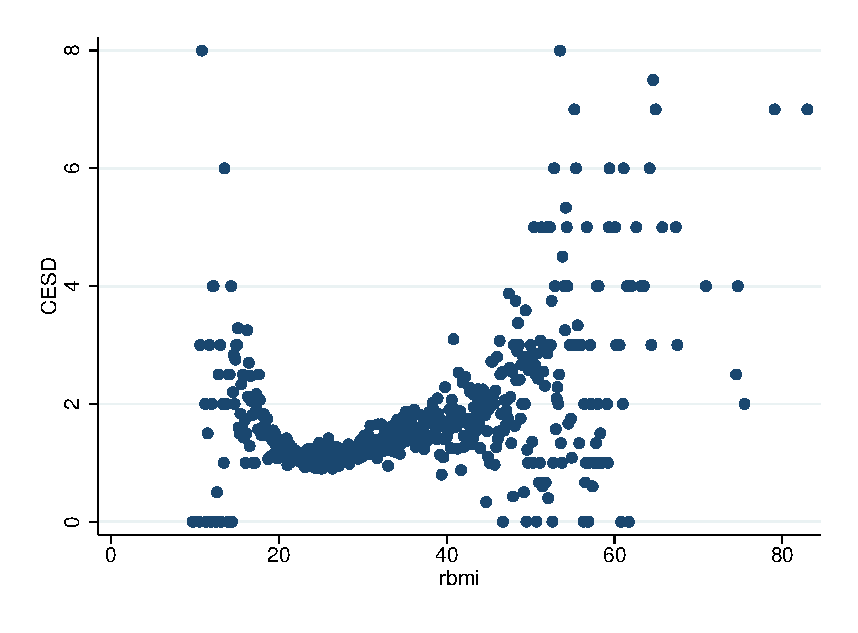
\includegraphics[width=0.6\paperwidth]{../proj/fig/cesd.eps}}
\caption{Mean depression as a function of the BMI}
\label{fig:cesd}
\end{figure}


\begin{figure}[H]
\makebox[\textwidth][c]{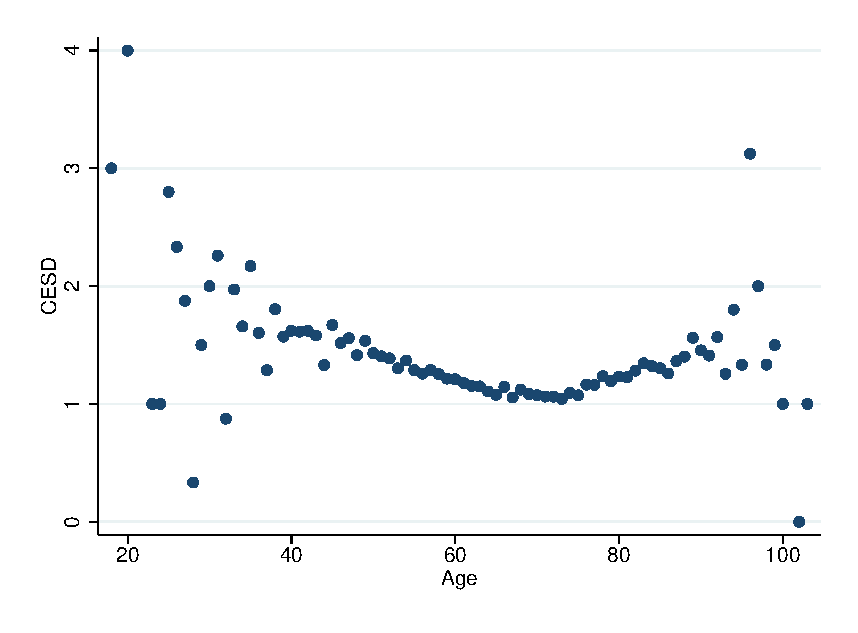
\includegraphics[width=0.6\paperwidth]{../proj/fig/agecesd.eps}}
\caption{Mean depression score as a function of the age}
\label{fig:agecesd}
\end{figure}



\begin{figure}[H]
\makebox[\textwidth][c]{\includegraphics[width=0.6\paperwidth]{../proj/fig/agebmi.eps}}
\caption{Mean bmi as a function of the age}
\label{fig:agebmi}
\end{figure}

\begin{figure}[H]
\makebox[\textwidth][c]{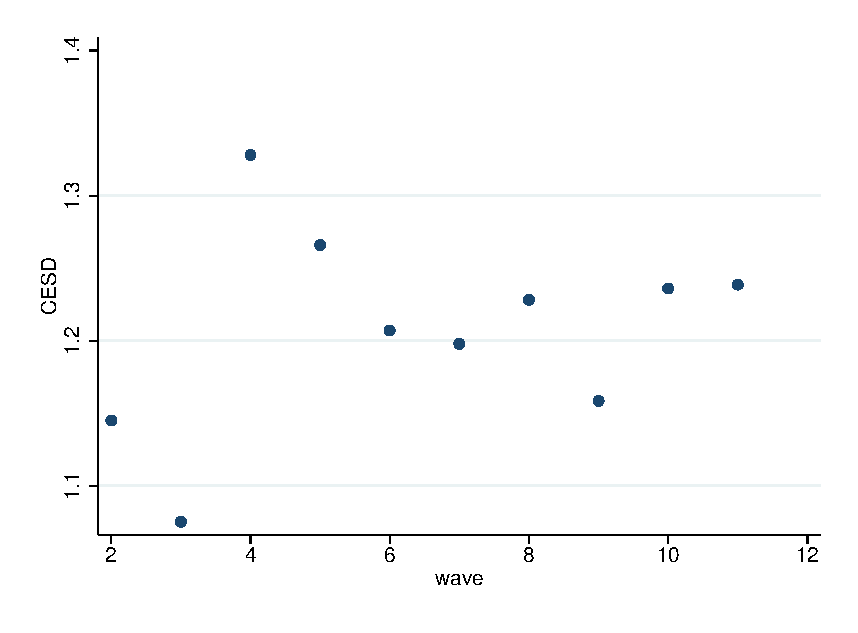
\includegraphics[width=0.6\paperwidth]{../proj/fig/wavecesd.eps}}
\caption{Mean depression score as a function of the wave}
\label{fig:wavecesd}
\end{figure}

\begin{figure}[H]
\makebox[\textwidth][c]{\includegraphics[width=0.6\paperwidth]{../proj/fig/wavebmi.eps}}
\caption{Mean bmi as a function of the wave}
\label{fig:wavebmi}
\end{figure}


\subsection{Tables}

\subsubsection{Descriptive Analysis}

\begin{figure}[H]
\makebox[\textwidth][c]{\includegraphics[width=0.6\paperwidth]{../proj/matlab/2.pdf}}
\caption{Visual representation of the obtained coefficients for CESD and both sexes, scaled by the proportion of the population in the category }
\label{fig:results2}
\end{figure}



\begin{table}[H]
\centering
{
\def\sym#1{\ifmmode^{#1}\else\(^{#1}\)\fi}
\begin{tabular}{l*{3}{c}}
\hline\hline
                    &\multicolumn{1}{c}{(1)}&\multicolumn{1}{c}{(2)}&\multicolumn{1}{c}{(3)}\\
                    &\multicolumn{1}{c}{\shortstack{weightProblems\\reg}}&\multicolumn{1}{c}{\shortstack{weightProblems\\ivreg}}&\multicolumn{1}{c}{\shortstack{weightProblems\\ivprobit marginal}}\\
\hline
CESD depression score&      0.0168\sym{***}&      0.0491\sym{***}&      0.0458\sym{***}\\
                    &   (0.00164)         &   (0.00809)         &   (0.00751)         \\
[1em]
Male x CESD         &     -0.0190\sym{***}&     -0.0665\sym{***}&     -0.0619\sym{***}\\
                    &   (0.00244)         &    (0.0110)         &    (0.0110)         \\
[1em]
Male                &       0.165\sym{***}&       0.221\sym{***}&       0.214\sym{***}\\
                    &   (0.00812)         &    (0.0149)         &    (0.0137)         \\
[1em]
has smoked          &      -0.150\sym{***}&      -0.166\sym{***}&      -0.153\sym{***}\\
                    &    (0.0120)         &    (0.0126)         &    (0.0109)         \\
[1em]
Spouse has smoked   &     0.00324         &    -0.00109         &    -0.00137         \\
                    &   (0.00782)         &   (0.00798)         &   (0.00788)         \\
[1em]
Male x has smoked   &     -0.0288         &    -0.00317         &     -0.0150         \\
                    &    (0.0159)         &    (0.0168)         &    (0.0154)         \\
[1em]
Age                 &    -0.00631\sym{***}&    -0.00620\sym{***}&    -0.00605\sym{***}\\
                    &  (0.000521)         &  (0.000523)         &  (0.000522)         \\
[1em]
Spouse's Age        &   -0.000712         &   -0.000807         &   -0.000770         \\
                    &  (0.000514)         &  (0.000516)         &  (0.000513)         \\
\hline
Observations        &      100600         &      100600         &      100600         \\
Education Control   &         Yes         &         Yes         &         Yes         \\
Wave Control        &         Yes         &         Yes         &         Yes         \\
\hline\hline
\multicolumn{4}{l}{\footnotesize \footnotesize Standard errors clustered by id in parentheses}\\
\multicolumn{4}{l}{\footnotesize \footnotesize \sym{*} \(p<0.05\), \sym{**} \(p<0.01\), \sym{***} \(p<0.001\)}\\
\end{tabular}
}

\caption{Regression results over the weight problems dependent variable}
\label{tab:weightProblems}
\end{table}

\begin{table}[H]
\centering
{
\def\sym#1{\ifmmode^{#1}\else\(^{#1}\)\fi}
\begin{tabular}{l*{3}{c}}
\hline\hline
                    &\multicolumn{1}{c}{(1)}&\multicolumn{1}{c}{(2)}&\multicolumn{1}{c}{(3)}\\
                    &\multicolumn{1}{c}{\shortstack{overweight\\reg}}&\multicolumn{1}{c}{\shortstack{overweight\\ivreg}}&\multicolumn{1}{c}{\shortstack{overweight\\ivprobit marginal}}\\
\hline
CESD depression score&      0.0152\sym{***}&      0.0445\sym{***}&      0.0412\sym{***}\\
                    &   (0.00168)         &   (0.00825)         &   (0.00769)         \\
[1em]
Male x CESD         &     -0.0190\sym{***}&     -0.0646\sym{***}&     -0.0599\sym{***}\\
                    &   (0.00249)         &    (0.0111)         &    (0.0113)         \\
[1em]
Male                &       0.176\sym{***}&       0.229\sym{***}&       0.222\sym{***}\\
                    &   (0.00823)         &    (0.0151)         &    (0.0140)         \\
[1em]
has smoked          &      -0.176\sym{***}&      -0.190\sym{***}&      -0.175\sym{***}\\
                    &    (0.0123)         &    (0.0128)         &    (0.0112)         \\
[1em]
Spouse has smoked   &     0.00248         &    -0.00135         &    -0.00174         \\
                    &   (0.00795)         &   (0.00810)         &   (0.00801)         \\
[1em]
Male x has smoked   &     -0.0123         &      0.0121         &    -0.00267         \\
                    &    (0.0162)         &    (0.0171)         &    (0.0156)         \\
[1em]
Age                 &    -0.00687\sym{***}&    -0.00677\sym{***}&    -0.00659\sym{***}\\
                    &  (0.000533)         &  (0.000535)         &  (0.000536)         \\
[1em]
Spouse's Age        &   -0.000868         &   -0.000961         &   -0.000924         \\
                    &  (0.000524)         &  (0.000525)         &  (0.000524)         \\
\hline
Observations        &      100600         &      100600         &      100600         \\
Education Control   &         Yes         &         Yes         &         Yes         \\
Wave Control        &         Yes         &         Yes         &         Yes         \\
\hline\hline
\multicolumn{4}{l}{\footnotesize \footnotesize Standard errors clustered by id in parentheses}\\
\multicolumn{4}{l}{\footnotesize \footnotesize \sym{*} \(p<0.05\), \sym{**} \(p<0.01\), \sym{***} \(p<0.001\)}\\
\end{tabular}
}

\caption{Regression results over the overweight dependent variable}
\label{tab:overweight}
\end{table}

\begin{table}[H]
\centering
{
\def\sym#1{\ifmmode^{#1}\else\(^{#1}\)\fi}
\begin{tabular}{l*{3}{c}}
\hline\hline
                    &\multicolumn{1}{c}{(1)}&\multicolumn{1}{c}{(2)}&\multicolumn{1}{c}{(3)}\\
                    &\multicolumn{1}{c}{\shortstack{obese\\reg}}&\multicolumn{1}{c}{\shortstack{obese\\ivreg}}&\multicolumn{1}{c}{\shortstack{obese\\ivprobit marginal}}\\
\hline
CESD depression score&      0.0185\sym{***}&      0.0555\sym{***}&      0.0497\sym{***}\\
                    &   (0.00168)         &   (0.00794)         &   (0.00683)         \\
[1em]
Male x CESD         &    -0.00653\sym{*}  &     -0.0317\sym{**} &     -0.0289\sym{**} \\
                    &   (0.00259)         &    (0.0111)         &    (0.0103)         \\
[1em]
Male                &      0.0336\sym{***}&      0.0688\sym{***}&      0.0636\sym{***}\\
                    &   (0.00781)         &    (0.0145)         &    (0.0137)         \\
[1em]
has smoked          &      -0.150\sym{***}&      -0.166\sym{***}&      -0.167\sym{***}\\
                    &   (0.00995)         &    (0.0106)         &    (0.0113)         \\
[1em]
Spouse has smoked   &      0.0124         &     0.00629         &     0.00580         \\
                    &   (0.00790)         &   (0.00799)         &   (0.00763)         \\
[1em]
Male x has smoked   &      0.0123         &      0.0286\sym{*}  &      0.0301         \\
                    &    (0.0134)         &    (0.0145)         &    (0.0157)         \\
[1em]
Age                 &    -0.00720\sym{***}&    -0.00706\sym{***}&    -0.00687\sym{***}\\
                    &  (0.000497)         &  (0.000498)         &  (0.000479)         \\
[1em]
Spouse's Age        &   -0.000264         &   -0.000291         &   -0.000445         \\
                    &  (0.000493)         &  (0.000495)         &  (0.000473)         \\
\hline
Observations        &      100600         &      100600         &      100600         \\
Education Control   &         Yes         &         Yes         &         Yes         \\
Wave Control        &         Yes         &         Yes         &         Yes         \\
\hline\hline
\multicolumn{4}{l}{\footnotesize \footnotesize Standard errors clustered by id in parentheses}\\
\multicolumn{4}{l}{\footnotesize \footnotesize \sym{*} \(p<0.05\), \sym{**} \(p<0.01\), \sym{***} \(p<0.001\)}\\
\end{tabular}
}

\caption{Regression results over the obese dependent variable}
\label{tab:obese}
\end{table}

\begin{table}[H]
\centering
{
\def\sym#1{\ifmmode^{#1}\else\(^{#1}\)\fi}
\begin{tabular}{l*{3}{c}}
\hline\hline
                    &\multicolumn{1}{c}{(1)}&\multicolumn{1}{c}{(2)}&\multicolumn{1}{c}{(3)}\\
                    &\multicolumn{1}{c}{\shortstack{morbidlyObese\\reg}}&\multicolumn{1}{c}{\shortstack{morbidlyObese\\ivreg}}&\multicolumn{1}{c}{\shortstack{morbidlyObese\\ivprobit marginal}}\\
\hline
CESD depression score&     0.00619\sym{***}&      0.0165\sym{***}&     0.00997\sym{***}\\
                    &  (0.000816)         &   (0.00330)         &   (0.00249)         \\
[1em]
Male x CESD         &    -0.00152         &    -0.00890\sym{*}  &    -0.00168         \\
                    &   (0.00115)         &   (0.00403)         &   (0.00367)         \\
[1em]
Male                &    -0.00887\sym{***}&     0.00132         &    -0.00948         \\
                    &   (0.00255)         &   (0.00512)         &   (0.00509)         \\
[1em]
has smoked          &     -0.0299\sym{***}&     -0.0344\sym{***}&     -0.0321\sym{***}\\
                    &   (0.00369)         &   (0.00405)         &   (0.00442)         \\
[1em]
Spouse has smoked   &     0.00843\sym{**} &     0.00671\sym{*}  &     0.00610\sym{*}  \\
                    &   (0.00314)         &   (0.00315)         &   (0.00273)         \\
[1em]
Male x has smoked   &     0.00723         &      0.0119\sym{*}  &     0.00253         \\
                    &   (0.00417)         &   (0.00470)         &   (0.00608)         \\
[1em]
Age                 &    -0.00155\sym{***}&    -0.00151\sym{***}&    -0.00152\sym{***}\\
                    &  (0.000190)         &  (0.000189)         &  (0.000166)         \\
[1em]
Spouse's Age        &   0.0000776         &   0.0000691         &  -0.0000860         \\
                    &  (0.000184)         &  (0.000183)         &  (0.000164)         \\
\hline
Observations        &      100600         &      100600         &      100600         \\
Education Control   &         Yes         &         Yes         &         Yes         \\
Wave Control        &         Yes         &         Yes         &         Yes         \\
\hline\hline
\multicolumn{4}{l}{\footnotesize \footnotesize Standard errors clustered by id in parentheses}\\
\multicolumn{4}{l}{\footnotesize \footnotesize \sym{*} \(p<0.05\), \sym{**} \(p<0.01\), \sym{***} \(p<0.001\)}\\
\end{tabular}
}

\caption{Regression results over the morbidly obese dependent variable}
\label{tab:morbidlyObese}
\end{table}

\begin{table}[H]
\centering
{
\def\sym#1{\ifmmode^{#1}\else\(^{#1}\)\fi}
\begin{tabular}{l*{3}{c}}
\hline\hline
                    &\multicolumn{1}{c}{(1)}&\multicolumn{1}{c}{(2)}&\multicolumn{1}{c}{(3)}\\
                    &\multicolumn{1}{c}{\shortstack{obese\\reg}}&\multicolumn{1}{c}{\shortstack{obese\\ivreg}}&\multicolumn{1}{c}{\shortstack{obese\\ivprobit marginal}}\\
\hline
wave==3             &      0.0219\sym{***}&      0.0232\sym{***}&      0.0251\sym{***}\\
                    &   (0.00342)         &   (0.00351)         &   (0.00394)         \\
[1em]
wave==4             &      0.0459\sym{***}&      0.0398\sym{***}&      0.0447\sym{***}\\
                    &   (0.00401)         &   (0.00437)         &   (0.00480)         \\
[1em]
wave==5             &      0.0620\sym{***}&      0.0567\sym{***}&      0.0619\sym{***}\\
                    &   (0.00438)         &   (0.00466)         &   (0.00513)         \\
[1em]
wave==6             &      0.0873\sym{***}&      0.0827\sym{***}&      0.0878\sym{***}\\
                    &   (0.00483)         &   (0.00503)         &   (0.00550)         \\
[1em]
wave==7             &      0.0959\sym{***}&      0.0915\sym{***}&      0.0962\sym{***}\\
                    &   (0.00490)         &   (0.00510)         &   (0.00553)         \\
[1em]
wave==8             &       0.126\sym{***}&       0.121\sym{***}&       0.124\sym{***}\\
                    &   (0.00525)         &   (0.00550)         &   (0.00595)         \\
[1em]
wave==9             &       0.146\sym{***}&       0.142\sym{***}&       0.145\sym{***}\\
                    &   (0.00560)         &   (0.00578)         &   (0.00618)         \\
[1em]
wave==10            &       0.161\sym{***}&       0.155\sym{***}&       0.153\sym{***}\\
                    &   (0.00539)         &   (0.00565)         &   (0.00601)         \\
[1em]
wave==11            &       0.173\sym{***}&       0.167\sym{***}&       0.165\sym{***}\\
                    &   (0.00561)         &   (0.00589)         &   (0.00625)         \\
\hline
Observations        &      100600         &      100600         &      100600         \\
Other variables ommitted&         Yes         &         Yes         &         Yes         \\
\hline\hline
\multicolumn{4}{l}{\footnotesize \footnotesize Standard errors clustered by id in parentheses}\\
\multicolumn{4}{l}{\footnotesize \footnotesize \sym{*} \(p<0.05\), \sym{**} \(p<0.01\), \sym{***} \(p<0.001\)}\\
\end{tabular}
}

\caption{Regression explaining obesity only showing the wave control}
\label{tab:wave}
\end{table}

\begin{table}[H]
\centering
{
\def\sym#1{\ifmmode^{#1}\else\(^{#1}\)\fi}
\begin{tabular}{l*{3}{c}}
\hline\hline
                    &\multicolumn{1}{c}{(1)}&\multicolumn{1}{c}{(2)}&\multicolumn{1}{c}{(3)}\\
                    &\multicolumn{1}{c}{\shortstack{obese\\reg}}&\multicolumn{1}{c}{\shortstack{obese\\ivreg}}&\multicolumn{1}{c}{\shortstack{obese\\ivprobit marginal}}\\
\hline
raeduc==2           &    0.000891         &      0.0104         &     0.00733         \\
                    &    (0.0154)         &    (0.0156)         &    (0.0141)         \\
[1em]
raeduc==3           &     -0.0196\sym{*}  &   -0.000817         &    -0.00283         \\
                    &   (0.00865)         &   (0.00973)         &   (0.00916)         \\
[1em]
raeduc==4           &     -0.0452\sym{***}&     -0.0240\sym{*}  &     -0.0267\sym{**} \\
                    &   (0.00920)         &    (0.0105)         &    (0.0100)         \\
[1em]
raeduc==5           &      -0.124\sym{***}&     -0.0974\sym{***}&      -0.101\sym{***}\\
                    &   (0.00906)         &    (0.0113)         &    (0.0116)         \\
\hline
Observations        &      100600         &      100600         &      100600         \\
Other variables ommitted&         Yes         &         Yes         &         Yes         \\
\hline\hline
\multicolumn{4}{l}{\footnotesize \footnotesize Standard errors clustered by id in parentheses}\\
\multicolumn{4}{l}{\footnotesize \footnotesize \sym{*} \(p<0.05\), \sym{**} \(p<0.01\), \sym{***} \(p<0.001\)}\\
\end{tabular}
}

\caption{Regression explaining obesity only showing the education control}
\label{tab:educ}
\end{table}

\begin{table}[H]
\centering
{
\def\sym#1{\ifmmode^{#1}\else\(^{#1}\)\fi}
\begin{tabular}{l*{2}{c}}
\hline\hline
                    &\multicolumn{1}{c}{(1)}&\multicolumn{1}{c}{(2)}\\
                    &\multicolumn{1}{c}{\shortstack{obese\\reg}}&\multicolumn{1}{c}{\shortstack{obese\\ivreg}}\\
\hline
CESD depression score&      0.0189\sym{***}&      0.0480\sym{***}\\
                    &   (0.00132)         &   (0.00578)         \\
\hline
Observations        &      100600         &      100600         \\
\hline\hline
\multicolumn{3}{l}{\footnotesize \footnotesize Standard errors clustered by id in parentheses}\\
\multicolumn{3}{l}{\footnotesize \footnotesize \sym{*} \(p<0.05\), \sym{**} \(p<0.01\), \sym{***} \(p<0.001\)}\\
\end{tabular}
}

\caption{Simplest obese regression}
\label{tab:bias}
\end{table}

\end{document}